\section{Multiplexing}
    
    Quando la larghezza di banda di un canale trasmissivo è maggiore della larghezza di banda effettivamente necessaria, il canale può essere condivisdo da più trasmissioni contemporaneamente.
    
    \vspace{3mm}
    
    \textbf{Il multiplexing è definito come l'insieme delle tecniche che ottimizzano l'utilizzo di un canale di comunicazione, permettono la trasmissione simultanea di più segnali su un singolo canale di comunicazione.} 
    Avendo un mezzo trasmissivo e dei dati da inviare, talvolta la soluzione più efficiente - canale permettendo - potrebbe essere inviare più segnali alla volta.
    
    L'idea è utilizzare canali con una larghezza di banda grande per potere trasportare contemporaneamente dati di più canali logici.
    
    \vspace{3mm}
    
    Ad esempio, si ponga il caso di dover spedire dati a 3Mbps su un canale a 10Mbps: in questo caso, sprecheremmo 7Mbps. Potremmo dunque inviare contemporaneamente 3 comunicazioni a 3 Mbps, sprecandone solo 1.
    
    \begin{center}
        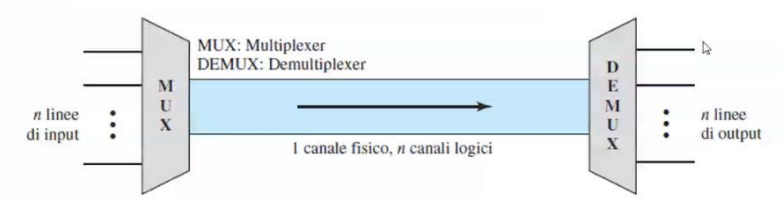
\includegraphics[scale=0.6]{images/Multiplexing.png}
    \end{center}
    
    In un sistema con multiplexing vi è 1 canale fisico e $n$ linee trasmissive. Volendo inviare $n$ segnali su questo singolo canale fisico, sarà necessario scomporre logicamente il canale fisico in $n$ parti, ognuna corrispondente ad una linea trasmissiva. Si parla dunque di scomposizione logica per la quale un canale fisico viene rappresentato con più canali logici. 
    
    Il multiplexer è un dispositivo che si occupa di prendere i dati sui canali logici e spedirli sul canale fisico, aggregandoli. 
    
    Il demultiplexer effettua l'operazione inversa, e cioè scomporre i dati dal singolo canale fisico a più canali logici.
    
    \subsection{Tecniche di Multiplexing}
        Esistono tre tecniche generali per implementare il multiplexing. Le prime due si utilizzano per segnali analogici, la terza per segnali digitali. La seconda riguarda, in particolare, le fibbre ottiche.
    
        \begin{itemize}
            \item 
                \textbf{FDM (Divisione di Frequenza).} E' una tecnica di multiplexing per  segnali analogici. I segnali dei singoli canali logici vengono modulati usando frequenze portanti diverse; i segnali così ottenuti vengono combinati in un singolo segnale composto che può essere trasportato sul collegamento. Le frequenze portanti vengono scelte in modo tale che i segnali modulanti non interferiscano l'uno con l'altro.
                
                Ogni canale è pensato per una singola frequenza. Si prendono i segnali in input dai singoli canali logici, e vengono modulati usando delle frequenze portanti diverse.
                
                \begin{center}
                    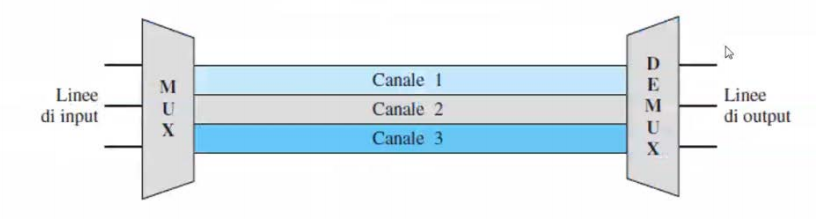
\includegraphics[scale=0.6]{images/FDM.png}
                \end{center}
                
                In fase di \textit{multiplexing}, ogni canale logico genera un segnale sulle stesse frequenze. All'interno del multiplexer questi segnali simili vengono modulati utilizzando segnali portanti di frequenza diversa. I segnali che derivano da ognuna delle modulazioni vengono combinati per creare un singolo segnale composto, per essere poi inviato lungo il mezzo trasmissivo.
                
                \begin{center}
                    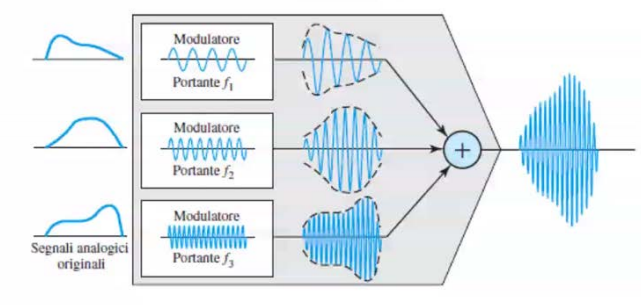
\includegraphics[scale=0.6]{images/FDM_Mult.png}
                \end{center}
                
                In fase di \textit{demultiplexing}, il demultiplexer utilizza una serie di filtri per scomporre il segnale composto ricevuto nei singoli segnali originali. Ciascun segnale viene fatto passare attraverso un demodulatore che supera il segnale che rappresenta i dati originali dal segnale portante usato per modularlo.
            
                \begin{center}
                    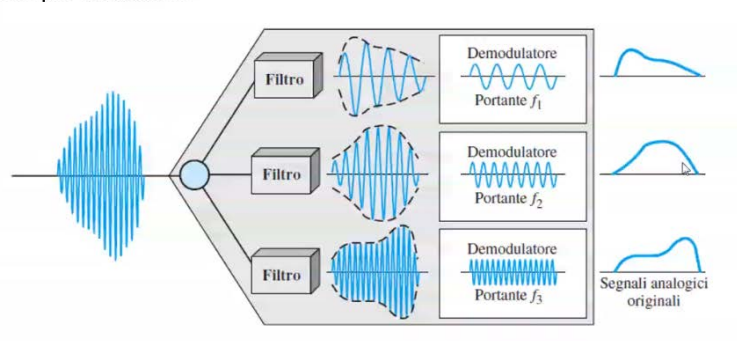
\includegraphics[scale=0.6]{images/FDM_Demult.png}
                \end{center}
            
            \item
                \textbf{WDM (Divisione di Lunghezza d'Onda).} Tecnica di multiplexing per segnali ottici, utilizza per i cavi in fibra ottica a velocità elevata. Utilizza un meccanismo simile al \textit{prisma}. Ogni segnale può essere visto come una sorgente luminosa; il prisma, infatti permette di accorpare i segnali in un'unica sorgente luminosa.
                
                \begin{center}
                    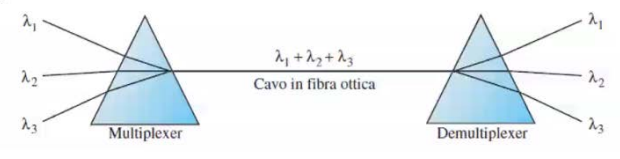
\includegraphics[scale=0.6]{images/WDM.png}
                \end{center}
                
                La modulazione è effettuata sulla lunghezza d'onda del segnale; è una tecnica complessa ma l'idea di base è semplice: si combinano varie sorgenti di luce in un singolo segnale luminoso (multiplexer) o si fa l'esatto opposto (demultiplexer). Le operazioni di raggruppamento e di divisione dei segnal iluminosi possono essere effettuate mediante un prisma, che devia un raggio luminoso in base all'angolo di incidenza e alla frequenza.
             
            \item
                \textbf{TDM (Divisione di Tempo).} Progettato per condividere un canale digitale. Invece di condividere una porzione della larghezza di banda, come nel FDM, esso condivide il tempo di utilizzo del collegamento. Ogni canale logico occupa un intervallo di tempo in maniera sincrona o statistica.
                
                Siccome abbiamo informazioni digitali, che hanno valori discreti (motivo per cui non si può ragionare in termini di modulazioni), piuttosto che condividere livelli di frequenza del segnale, si può condividere - a turno - il tempo di utilizzo del segnale stesso.
                
                Si immagina di suddividere la fase di trasmissione dei dati in vari intervalli; per ogni intervallo, a turno, si decidono quali segnali sui canali logici devono essere inviati.
                
                \begin{center}
                    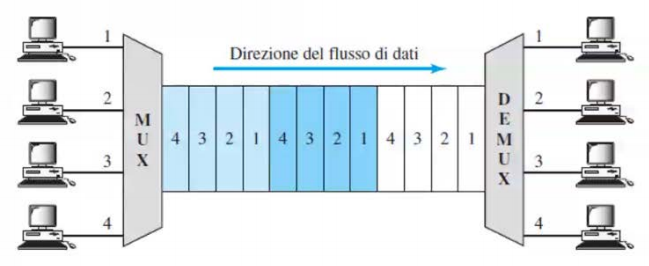
\includegraphics[scale=0.6]{images/TDM.png}
                \end{center}
                
                \begin{itemize}
                    \item 
                        Nel \textbf{TDM sincrono}, l'utilizzo del collegamento fisico viene suddiviso in intervalli di tempo. Il canale viene sfruttato a turno da ogni singolo canale logico. 
                        
                        La grandezza dell'intervallo (assegnato staticamente) in sé è un parametro dello schema, che determina il numero di bit che si possono spedire in quell'intervallo. La velocità del collegamento è $n$ volte quella dei canali. 
                        
                        I dati provenienti da ognuno dei canali vengono spediti a turno, seguendo un ordine prestabilito. Gli intervalli sono assegnati staticamente; se un canale non ha dati, l'intervallo viene sprecato.
                    
                        \begin{center}
                            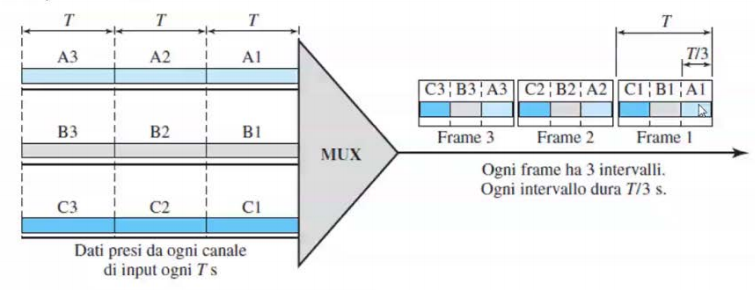
\includegraphics[scale=0.6]{images/TDM_Sincrono.png}
                        \end{center}
                    
                        In particolare, il TDM sincrono può essere \textit{multilivello} (utilizzato quando la velocità delle linee di input sono l'una multiplo dell'altra) e \textit{multiturno} (alloca più di un turno ad un canale che è più veloce degli altri. Le velocità devono essere tutte multiple di un'unità di base - in pratica, si accorpano i segnali per sfruttare la capacità del mezzo).
                        
                        \vspace{3mm}
                        
                        La suddivisione in frame è ideale. Abbiamo bisogno, però, di un'informazione di sincronizzazione, per capire quando l'intervallo corrispondente ad un certo frame è terminato. Si stabilisce uno \textit{schema di sincronizzazione}, ossia una sequenza di bit inseriti in un frame. 
                        
                        Ad esempio, $101$ (con $1$ alla fine del primo frame, $0$ alla fine del secondo, $1$ alla fine del terzo) è una sottosequenza che rappesenta - a partire dall'inizio dell'invio dei dati - uno schema di sincronizzazione, che permette - attraverso delle tecniche di ricostruzione - di far capire al destinatario che si è ricevuti esattamente tre frame.
                        
                        \vspace{3mm}
                        
                        Il vantaggio del TDM sincrono è la facilità di individuazione dei singoli canali; lo svantaggio è lo spreco di intervalli.
                    
                    \item
                        Nel \textbf{TDM statistico}, \textbf{gli intervalli sono assegnati dinamicamente}. Se un canale non ha dati, l'intervallo viene usato da un altro canale.
                        
                        \vspace{3mm}
                        
                        Il vantaggio del TDM statistico è che usa sempre gli intervalli; lo svantaggio giace nella difficoltà nel determinare l'identità del singolo canale logico.
                \end{itemize}
        \end{itemize}